% Chapter 4

\chapter{Experiments}
\label{Chapter4}

In order to assess the quality of the proposed methodology, described in Section
\ref{sec:method}, we tested it on several commonly adopted benchmarks and against
different baseline methods that will be detailed in the following sections.

\section{Datasets}
\label{subsec:datasets}

The experiments were conducted on five real-world applications datasets, namely:
AIDS \cite{Weislow19041989}, CAS\footnote{http://cheminformatics.org/datasets/bursi/},
CPDB \cite{journals/jcisd/HelmaCKR04}, GDD \cite{dobson2003}, and NCI1 \cite{journals/kais/WaleWK08}.
All these datasets contains chemical and molecular particles encoded in graph form,
all the nodes are labelled and none have self loops, that is an edge going out
and into the same node.
The AIDS Antiviral Screen dataset contains chemical compounds, labelled according to
their antiviral activity; CAS and CPDB are dataset of mutagenic
compounds; NCI1 consists of chemical compounds screened for activity against 
non-small lung cancer cells; GDD is composed of X-ray crystal structures of
proteins represented as graphs.
Some statistics about these datasets are reported in table~\ref{table:datasets}.

    \begin{table}[ht]
        \centering
        \begin{tabular}{|r|r|r|r|r|}
            \hline
            Dataset & n. of graphs & sample split & avg nodes & avg edges \\ \hline
            AIDS    & 1503         & 28.07        & 58.90     & 61.40     \\ \hline      
            CAS     & \textbf{4337} & 55.36        & 29.90     & 30.90     \\ \hline      
            CPDB    &  684         & 49.85        & 14.10     & 14.60     \\ \hline      
            GDD     & 1503         & 58.65        & 284.31    & \textbf{2862.63}   \\ \hline      
            NCI1    & 1503         & 50.04        & 29.87     & 32.30     \\ \hline      
        \end{tabular}
        \caption{Statistics about the datasets employed in the experiments: number
        of graphs, labels percentage among samples, average number of nodes, average
        number of edges. It is clear from this table that the CAS and NCI1 datasets
        are the bigger ones while the GDD holds the most complex graphs either in
        terms of topography and processing. Furthermore the AIDS dataset turns out
        to be quite unbalanced in terms of labels distribution \cite{rtesselli}.}
        \label{table:datasets}
    \end{table}

%----------------------------------------------------------------------------------------

\section{Experiments description}
\label{sec:description}

% add more motivations behind these experiments.
The $k$ parameter of the cross-validation has been fixed at 10 since this value
already provides good statistical significance while helping containing the bias
skewing during the training phase.
Moreover, the whole routine has been run ten times with ten different splits of the
data in order to mitigate the high variance derived during the testing phase due to the
chosen value of $k$.

The original kernel combinations selected for this study were:
\begin{enumerate}
    \item the $ODDK_{ST}$ (Section \ref{subsubsec:odd}) and $TCK_{ST}$ (Section \ref{subsec:context}) graph kernels,
    \item the $ODDK_{ST+}$ (Section \ref{subsubsec:odd}) and $TCK_{ST+}$ (Section \ref{subsec:context}) graph kernels,
    \item the $WL$ (Section \ref{subsubsec:fs}) fast subtree and $WLC$ (Section \ref{subsec:context}) graph kernels.
\end{enumerate}

For each combination a separated set of experiment was conducted, while maintaining
the same structure, of which a detailed breakdown will be given in Table \ref{table:structure}.

\begin{table}[ht]
    \centering
    \begin{tabular}{|l|l|l|}
        \hline
        n. & method & kernels \\
        \hline
        1 & EasyMKL & $K$ and $K'$ \\
        \hline
        2 & EasyMKL & $K'$ \\
        \hline
        3 & EasyMKL & $K$ \\
        \hline
    \end{tabular}
    \caption{Structure of the main experiments. Kernels $K$ and $K'$ refer
    to the version without and with contexts for each combination respectively.
    These kernels generated a set of matrices each, according to the technique
    described in Section \ref{subsec:features} which were concatenated as a list
    to be given in input to EasyMKL.}
    \label{table:structure}
\end{table}

The hyper-parameter selection process for the kernels has been embedded
into the MKL learning phase so each set of kernel matrices has been
pre-computed for each one of the possible combinations of parameters that would
otherwise have been used in a grid-search fashion.
For all the following experiments, the $\Lambda$ parameter of EasyMKL has been
validated from the set $\{0.0, 0.1,\dots,1.0\}$ during the cross-validation
routine.

\paragraph{The case of the GDD dataset:}
\label{par:gdd}
confirming the experience reported in \cite{rtesselli}, while working with the GDD
dataset and the $ODD$ kernels we had to limit the $h$ hyper-parameter to the set
$\{1,2,3\}$ because for heights greater than 3 the computational times of the
kernel matrices became prohibitive, due to the high complexity and magnitude
of the data structures contained in this dataset.


\subsection[$ODDK_{ST}$ and $TCK_{ST}$]{$\boldsymbol{ODDK_{ST}}$ and $\boldsymbol{TCK_{ST}}$}
The kernels used for this experiment were generated from the $ODDK$ kernels
in \cite{DBLP:conf/sdm/MartinoNS12, Navarin2015}, namely $ODDK_{ST}$, $TCK_{ST}$.
Since EasyMKL took care of weighing the individual kernels, the $\lambda$
parameters of the ODD kernels has been fixed to 1, while the $h$ parameter
values were in the set $\{1,\dots,10\}$.

\subsection[$ODDK_{ST+}$ and $TCK_{ST+}$]{$\boldsymbol{ODDK_{ST+}}$ and $\boldsymbol{TCK_{ST+}}$}
The kernels used for this experiment were generated from the $ODDK$ kernels
in \cite{dasanmartino2015exploiting, rtesselli}, namely $ODDK_{ST+}$, $TCK_{ST+}$.
Again, EasyMKL took care of weighing the individual kernels so the $\lambda$
parameters of the ODD kernels has been fixed to 1, while the $h$ parameter
values were the set $\{1,\dots,10\}$.
During the cross-validation routine, the $\Lambda$ parameter of EasyMKL has been
validated from the set $\{0.0, 0.1,\dots,1.0\}$.

\subsection[$WL$ and $WLC$]{$\boldsymbol{WLK}$ and $\boldsymbol{WLCK}$}
The kernels used for this experiment were generated from the $Fast~Subtree$ kernels
in \cite{NIPS2009_3813, rtesselli}, namely the $WL$ kernel and the $WLC$ kernel.
These two kernels only need to validate one hyper-parameter, that is $h$ the iterations
limit whose values were those in the set $\{1,\dots,10\}$.
During the cross-validation routine, the $\Lambda$ parameter of EasyMKL has been
validated from the set $\{0.0, 0.1,\dots,1.0\}$.

%----------------------------------------------------------------------------------------

\section{Baselines}
We compared our methodology with some baseline performances against the same datasets.
The chosen baselines were:
\begin{enumerate}
    \item a single kernel approach employing an SVM with the follwing kernels:
        \begin{enumerate}
            \item $TCK_{ST},~TCK_{ST+},~WLC$;
            \item $TCK_{ST},~TCK_{ST+},~WLC$ summed with their non-contextualized
                version respectively;
        \end{enumerate}
    \item the MKL approach described in Section \ref{subsec:parameters} with the kernels:
        \begin{enumerate}
            \item $ODDK_{ST}\text{ and }TCK_{ST}$, combined and by themselves;
            \item $ODDK_{ST+}\text{ and }TCK_{ST+}$, combined and by themselves;
            \item $WLK\text{ and }WLCK$, combined and by themselves.
        \end{enumerate}
\end{enumerate}
Moreover, for the first combination of the list ($ODDK_{ST}$ and $TCK_{ST}$)
we compared our results against those in \cite{gmkl}, i.e. EasyMKL.
Table \ref{table:baselines} describes the general structure of the experiments
designed with this aim.

\begin{table}[ht]
    \centering
    \begin{tabular}{|l|l|l|}
        \hline
        n. & method & kernels \\
        \hline
        4 & EasyMKL & $K$ and $K'$ \\
        \hline
        5 & EasyMKL & $K'$ \\
        \hline
        6 & EasyMKL & $K$ \\
        \hline
        7 & SVC & $K'$ \\
        \hline
        8 & SVC & $K'+K$ \\
        \hline
    \end{tabular}
    \caption{Structure of the baseline experiments. Kernels $K$ and $K'$ refer
    to the version without and with contexts for each combination respectively.
    These kernels generated a set of matrices each, according to the hyper-parameters
    grid, which were concatenated as a list to be given in input to EasyMKL or
    given individually to an instance of the SVC. The expression $K + K'$ refers
    to the fact that the two kernel were summed prior to be used.}
    \label{table:baselines}
\end{table}

\subsection{Baselines with the SVM classifier}

Each kernel function listed in the first point of the list in the previous section has 
been used to train a SVM classifier whose $C$ parameter was validated
in the set $\{10^{-4},10^{-3},\dots,10^3\}$
The kernel functions parameter where validaten from the sets:
\begin{itemize}
    \item for the kernels derived from the $ODD$ framework:
    \begin{itemize}
        \item $h=\{1,\dots,10\}$ and 
        \item $\lambda=\{0.1, 0.5, 0.8, 0.9, 1.0, 1.1, 1.2, 1.3, 1.4, 1.5, 1.8\}$,
    \end{itemize}
    \item for the kernels derived from the $WL$ framework:
    \begin{itemize}
        \item $h=\{1,\dots,10\}$.
    \end{itemize}
\end{itemize}
The parameter sets both for the kernels and the classifier were taken from \cite{rtesselli}.

\subsection{EasyMKL baselines}
These baselines basically replicates the three main experiments described in Section
\ref{sec:description} but without the features subdivision strategy described in
Section \ref{subsec:features}.
The kernels derived from the $ODD$ framework were calculated according to a parameters grid
composed from the sets:
\begin{itemize}
    \item $h=\{1,\dots,10\}$ and 
    \item $\lambda=\{0.1, 0.5, 0.8, 0.9, 1.0, 1.1, 1.2, 1.3, 1.4, 1.5, 1.8\}$,
\end{itemize}
both sets were taken from \cite{rtesselli}.
To calculate the kernels derived from the $WL$ framework had their only hyper-parameter validated
in the set $h=\{1,\dots,10\}$.
During the cross-validation routine, the $\Lambda$ parameter of EasyMKL has been
validated from the set $\{0.0, 0.1,\dots,1.0\}$.

%----------------------------------------------------------------------------------------

\section{Results and discussion}
\label{sec:results}

\subsection{Space resources requirements}
Given the large number of kernel matrices involved in the combination exepriments
we would like to detail the space resources requirements that these experiments
had (Table \ref{table:space}) with the above mentioned setup.
Here we show only the data concerning the $ODD$ kernels since the $WL$ kernels
generated a number of matrices an order of magnitude less than the former.

\begin{table}[ht]
    \centering\footnotesize
    \begin{tabular}{|l|l|r|r|r|r|r|r|}
        \hline
        n. & method [kernel(s)] & no. m. & AIDS & CAS & CPDB & GDD & NCI1 \\
        \hline
        1 & EasyMKL [$K$ and $K'$] & 130 & 5 GB & 34 GB & 3 GB & <2 GB & 29 GB \\
        \hline
        2 & EasyMKL [$K'$] & 65 & 3 GB & 19 GB & <2 GB & <1 GB & 17 GB \\
        \hline
        3 & EasyMKL [$K$] & 65 & 3 GB & 19 GB & <2 GB & <1 GB & 17 GB \\
        \hline
        4 & EasyMKL [$K$ and $K'$] & 220 & 10 GB & 56 GB & 5 GB & 3 GB & 48 GB \\
        \hline
        5 & EasyMKL [$K'$] & 110 & 5 GB & 32 GB & 2 GB & 1 GB & 24 GB \\
        \hline
        6 & EasyMKL [$K$] & 110 & 5 GB & 32 GB & 2 GB & 1 GB & 24 GB \\
        \hline
    \end{tabular}
    \caption{Memory occupation in GigaBytes for each dataset during the different
    experiments. The third column represent the number of kernel matrices given as
    input to the algorithm for each experiments: due to the reduced parameters grid,
    in experiment 1 a total of 130 matrices where computed for each dataset
    (18 for GDD, Paragraph \ref{par:gdd}), while for experiments 2 and 3 a total
    of 65 matrices for each dataset where computed (9 for GDD), from this data we
    can see that the number of matrices is almost halved using the proposed methodology.}
    \label{table:space}
\end{table}

Time resources requirements being a part of the proposed improvements will be given
in Section \ref{subsec:time_results}.

\subsection{Analysis of the computational times}
\label{subsec:time_results}

The plot in figure~\ref{fig:times} shows the relation between the computation times
for the $ODD_{ST}\text{ and }TCK_{ST}$ kernels combination on the benchmark datasets,
using Algorithm \ref{alg:incremental} detailed in Section \ref{sec:inc}.
See Section~\ref{subsec:datasets} for further details on the composition of each dataset.
From the data it is clear that the complexity of computing the kernel in an incremental
fashion does not grow with the number of kernels being computed. (DRAFT: needs more data?)

\begin{figure}[ht]
    \centering
    \includegraphics[scale=0.5]{Figures/kernel_times_log2}
    \caption{Times in seconds required to compute the kernels $ODD_{ST}$ and 
    $TCK_{ST}$ incrementally and sequentially on a selection of datasets. Time
    scale is logarithmic for the sake of presentation.}
    \label{fig:times}
\end{figure}

We now present an analysis of the computational time performances of our methodology
compared to the two baselines. To keep the results comparable we are here considering
only the results obtained by experiments 2, 6, and 8 (cfr. Table \ref{table:structure} and \ref{table:baselines});
this choice stem from the fact
that these experiments employ the same kernel function with three different methods.

\begin{figure}[ht]
    \centering
    \includegraphics[scale=0.7]{Figures/total_times}
    \caption{(DRAFT: this plot will be replicated for each one of the kernels combination)
        Plot of the times required to compute a full nested
        10-fold cross-validation on the benchmark datasets.
        The data shown here refers to experiments 2 (cyan), 6 (magenta) and 8 (yellow)
        i.e. with the kernel $TCK_{ST}$.
        (DRAFT: missing data has been plotted at 0; partial results from the other two datasets seem to agree with this plot)
    }
    \label{fig:datasetstimes}
\end{figure}

As one can see from Figure \ref{fig:datasetstimes}, our method performs generally
better or has comparable performances with respect to the single-kernel approach.
The only case where our method fares worse is with the GDD dataset and this can be
ascribed to the particular case which it represents, that is, due to the parameters
set limitation in this case we had way less matrices than we should have had and
this positively affects the single kernel method while being of no relevance for
EasyMKL, less influenced by the number of input matrices.
From this data we can finally conclude that our methodology is more susceptible
to dataset dimension variation (i.e. the number of records) while the single-kernel
method is ideed influenced by the same measure but it is even more influenced by
the dimensions of the parameters grid.

\begin{figure}[ht]
    \centering
    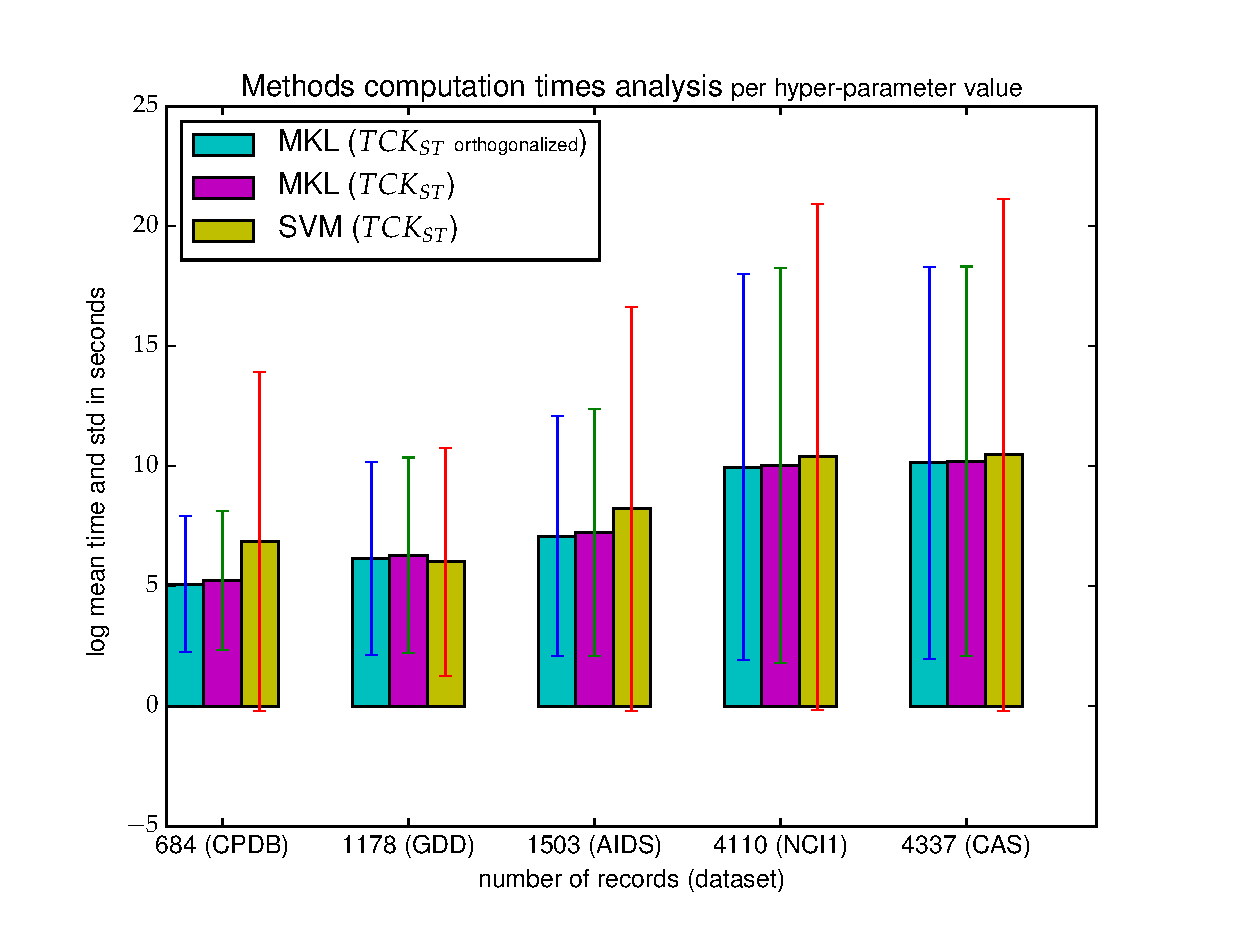
\includegraphics[scale=0.7]{Figures/method_times_avgstd}
    \caption{(DRAFT: is this plot useful? I think it shows the stableness of the algorithm
        over the whole computation and the fact that it is scarcely affected by the hyperparameter; missing data has been plotted at 0.)
        This plot shows the mean computation times among all the hyperparameter values,
        for each learning method and on all the benchmark datasets.
        Each point has the standard deviation among the same set of values plotted as well.
        (DRAFT: I'm not convinced on the presentation, I offset the three lines to highlight the
        standard deviation for each point but I think it could be confusing)
    }
        \label{fig:meantimes}
\end{figure}

\subsection{Analysis of the models performances}

Here we present the empirical results we got from the devised experiments described
in the previous sections.
Data is divided in three tables, one for each of the three combinations we chose.
Each table reports the ROAUC measure with the standard deviation measured with
a nested 10-fold cross validation. (DRAFT: should we substitute it with a 95\% confindence interval?)
ROAUC was chosen over accuracy to be able to compare the results obtained in \cite{gmkl}.

Looking at Table \ref{table:results_st}, it is immediately evident how the results
obtained by our methodology are always comparable when not even better with respect
to the baselines except in when considering the GDD dataset which, as mentioned in
Section \ref{subsec:time_results} is a rather peculiar case given the smaller dimensions
of the parameters grid considered.
While the results for experiment 2 seem in accordance with the results in \cite{gmkl},
the $TCK_{ST}$ (experiment 3) performs significantly worse with our MKL method than with
the SVM.
(DRAFT: experiments 4 and 6 have unexpected high performancs though.)

Table \ref{table:results_stp} present results in accordance with Table \ref{table:results_st}
beside the case of GDD in which apparently the $ODD_{ST+}$ and the version with
contextual informations are able to outperform the baselines while maintaining
comparable performance when used in combination (experiment 1).

From these results something that we can infer is the scarce improvment gained from
using one kernel and its contextualized version in combination with or without
the orthogonalization of the feature space.
All the obtained results shows that either both kernel fare at the same level or
one of them dominates the combination outcome: section \ref{sec:kca} will cover
more in detail this aspect.

\begin{landscape}
%    \begin{table}[ht]
%        \label{table:times}
%        \caption{(DRAFT) Times}
%    \end{table}

    \begin{table}[ht]\footnotesize
        \centering
        \begin{tabular}{|l|l|r|r|r|r|r|}
            \hline
            n. &method&CAS&NCI1&AIDS&CPDB&GDD\\
            \hline
            1& $MKL~(ODDK_{ST}, TCK_{ST})^*$&&&0.8632 $\pm$ 0.0034&\textbf{0.8632 $\pm$ 0.0038}&0.8528 $\pm$ 0.0022\\
            2& $MKL~(ODDK_{ST})^*$&&&0.8627 $\pm$ 0.0035&\textbf{0.8632 $\pm$  0.0029}&0.8543 $\pm$ 0.0024\\
            3& $MKL~(TCK_{ST})^*$&&&\textbf{0.8634 $\pm$ 0.0034}&0.8625 $\pm$ 0.0032&0.8458 $\pm$ 0.0021\\
            \hline
            4& $MKL~(ODDK_{ST}, TCK_{ST})$&0.8960 $\pm$  0.0012&0.9076 $\pm$ 0.0007&0.8468 $\pm$ 0.0042&0.8517 $\pm$ 0.0034&0.8612 $\pm$ 0.0018\\
            5& $MKL~(ODDK_{ST})$&0.8899 $\pm$ 0.0013&0.8976 $\pm$ 0.0010 &0.8388 $\pm$ 0.0044&0.8401 $\pm$ 0.0033&0.8013 $\pm$ 0.0019\\
            6& $MKL~(TCK_{ST})$&0.8954 $\pm$ 0.0013&0.9095 $\pm$ 0.0006&0.8487 $\pm$ 0.0040&0.8525 $\pm$ 0.0030&0.8617 $\pm$ 0.0022\\
            \hline
             & $MKL~(ODDK_{ST})^{**}$&\textbf{0.9049 $\pm$ 0.0008}&0.9144 $\pm$ 0.0008&0.8515 $\pm$ 0.0031&0.8564 $\pm$ 0.0056&0.8498 $\pm$ 0.0026\\
             & $SVM~(ODDK_{ST})^{**}$&0.8982 $\pm$ 0.0017&0.9069 $\pm$ 0.0010&0.8262 $\pm$ 0.0052&0.8442 $\pm$ 0.0067&0.8473 $\pm$ 0.0038\\
            \hline
            7& $SVM~(TCK_{ST} + ODDK_{ST})$&0.9010 $\pm$ 0.0011&0.9110 $\pm$ 0.0011&0.8323 $\pm$ 0.0065&0.8497 $\pm$ 0.0072&0.8627 $\pm$ 0.0018\\
            8& $SVM~(TCK_{ST})$&0.9006 $\pm$ 0.0013&\textbf{0.9150 $\pm$ 0.0011}&0.8225 $\pm$ 0.0067&0.8422 $\pm$ 0.0080&\textbf{0.8674 $\pm$ 0.0026}\\
            \hline
        \end{tabular}
        \caption{\footnotesize ROAUC results ($\pm$ standard deviation) relative to the combination
            of the $ODD_{ST}$ kernel with the $TCK_{ST}$ kernel. Results are
            obtained from a nested 10-fold cross validation. The first column is
            given as a reference to the experiment description given in Section
            \ref{sec:description}.
            The top part of the table contains the results of the main experiments
            while the bottom part those of the baselines.
            Lines marked with $^*$ refer to kernels whose feature space was split
            according to the technique exposed in \ref{subsec:features}.
            Lines marked with $^{**}$ refer to results obtained in \cite{gmkl}.
        }
        \label{table:results_st}
        \medskip

        \begin{tabular}{|l|l|r|r|r|r|r|}
            \hline
            n. & metodo&CAS&NCI1&AIDS&CPDB&GDD\\
            \hline
            1& $MKL (ODDK_{ST+}, TCK_{ST+})^*$&&&0.8632 $\pm$  0.0034&0.8632 $\pm$  0.0038&0.8528 $\pm$ 0.0022\\
            2& $MKL (ODDK_{ST+})^*$&&&0.8628 $\pm$  0.0036&0.8652 $\pm$ 0.0030&\textbf{0.8720 $\pm$ 0.0021}\\
            3& $MKL (TCK_{ST+})^*$&&&\textbf{0.8649 $\pm$  0.0030}&\textbf{0.8666 $\pm$  0.0038}&0.8711 $\pm$ 0.0018 \\
            \hline
            4& $MKL (ODDK_{ST+}, TCK_{ST+})$&&&0.8468 $\pm$ 0.0042&0.8517 $\pm$ 0.0034&0.8612 $\pm$ 0.0018\\
            5& $MKL (ODDK_{ST+})$&&&0.8489 $\pm$  0.0039&0.8461 $\pm$ 0.0036&0.8178 $\pm$ 0.0022\\
            6& $MKL (TCK_{ST+})$&&&0.8503 $\pm$  0.0038&0.8528 $\pm$ 0.0039&0.8645 $\pm$ 0.0018\\
            7& $SVM (TCK_{ST+} + ODDK_{ST+})$&0.9022 $\pm$ 0.0015 &0.9163 $\pm$ 0.0011&0.8256 $\pm$ 0.0068&0.8521 $\pm$ 0.0038&0.8570 $\pm$ 0.0043\\
            8& $SVM (TCK_{ST+})$&0.9008 $\pm$ 0.0017&0.9165 $\pm$ 0.0013&0.8222 $\pm$ 0.0067&0.8462 $\pm$ 0.0048&0.8588 $\pm$ 0.0028\\
            \hline
        \end{tabular}
        \caption{ROAUC results ($\pm$ standard deviation) relative to the combination
                of the $ODD_{ST+}$ kernel with the $TCK_{ST+}$ kernel. Results are
                obtained from a nested 10-fold cross validation. The nomenclature and
            results disposition is analogue to the one of Table \ref{table:results_st}.}
        \label{table:results_stp}
    \end{table}

%    \begin{table}[ht]
%        \label{table:results_wl}
%        \caption{ROAUC results ($\pm$ standard deviation) relative to the combination
%                of the $WL$ kernel with the $WLC$ kernel. Results are
%                obtained from a nested 10-fold cross validation. The nomenclature and
%            results disposition is analogue to the one of Table \ref{table:results_st}.}
%        \label{table:results_wl}
%    \end{table}
\end{landscape}

\section{Kernels Contribution Analysis}
\label{sec:kca}

\begin{figure}[ht]
    \centering
    \includegraphics[scale=0.7]{Figures/weightdist}
    \caption{(DRAFT: this plot is just an example of the available data for furhter analisys.
        I think we may be mainly interested in the experiments were two kernels are combined
        either with or without bucketization of the feature space.)
        Kernel weight distributions for the $TCK_{ST}$ kernel
    computed according to the full parameters grid, on the NCI1 dataset.
    The $x$ axis shows all the employed kernel matrices indexed by their hyperparameters
    values (ascending values left to right), the $y$ axis the weight values.
    Each plot refers to one run of the nested 10-fold cross-validation routine relative to one
    value for the $\Lambda$ parameter of EasyMKL. Weight values are the means between each of the inner
    cross-validation runs. The vertical lines highlight the kernel with the maximum weight for each value of $\Lambda$.}
        \label{fig:weightdist}
\end{figure}


